
%	Documentação do Trabalho Prático 1 de AEDSIII
%	@Sandro Miccoli
%
%	* Você pode identificar erros de grafia através do seguinte comando linux:
%		aspell --encoding="utf-8" -c -t=tex --lang="pt_BR" tp1.tex
%

\documentclass[12pt]{article}
\usepackage{sbc-template}
\usepackage{graphicx}
\usepackage{latexsym}
\usepackage{changepage}   % for the adjustwidth environment
\usepackage{subfigure}
\usepackage{times,amsmath,epsfig}
\usepackage{graphicx,url}
 \makeatletter
 \newif\if@restonecol
 \makeatother
 \let\algorithm\relax
 \let\endalgorithm\relax
\graphicspath{{./data/}}
\usepackage[lined,algonl,ruled]{algorithm2e}
\usepackage{multirow}
\usepackage[brazil]{babel}
\usepackage[utf8]{inputenc}
\usepackage{listings}

\usepackage{alltt}
\renewcommand{\ttdefault}{txtt}

\sloppy

<<<<<<< HEAD
\title{Programação Modular \\ Trabalho Prático 2: \\ Pôquer Chinês}

\author{Sandro Miccoli - 2009052409 - smiccoli@dcc.ufmg.br\\
		Frederico Figueiredo - 2010054371 - fredfig@dcc.ufmg.br}
=======
\title{Programação Modular \\ Trabalho Final \\ Visualização Interativa de Agentes Inteligentes}

\author{Daniel Diniz - 2008046090 - daniel.diniz@dcc.ufmg.br\\
		Diogo Santana - 2011054308 - diogo.santana@dcc.ufmg.br\\
		Frederico Figueiredo - 2010054371 - fredfig@dcc.ufmg.br\\
		Sandro Miccoli - 2009052409 - smiccoli@dcc.ufmg.br}
>>>>>>> Sandro

\address{Departamento de Ciência da Computação -- Universidade Federal de Minas Gerais (UFMG)\\
\\
\today}


\begin{document}

\maketitle


\begin{resumo}

<<<<<<< HEAD
Esse relatório descreve como foi implementado o jogo Pôquer Chinês, proposto como tema para o Trabalho Prático 2. A Seção \ref{introducao} introduz o problema proposto e dá uma visão geral da solução implementada. Cada seção irá descrever detalhes do sistema desenvolvido, abrangendo desde o planejamento (Seção \ref{planejamento}), as decisões de implementação (Seção \ref{implementacao}) e os testes realizados (Seção \ref{testes}). Finalmente concluímos (Seção \ref{conclusao}) a documentação com reflexões sobre o aprendizado durante a execução do trabalho.
=======
Esse relatório descreve como foi implementado a Visualização Interativa de Agentes Inteligentes, proposto como tema para o Trabalho Final. A Seção \ref{introducao} introduz o problema proposto e dá uma visão geral da solução implementada. Cada seção irá descrever detalhes do sistema desenvolvido, abrangendo desde o planejamento (Seção \ref{planejamento}), as decisões de implementação (Seção \ref{implementacao}) e os testes realizados (Seção \ref{testes}). Finalmente concluímos (Seção \ref{conclusao}) a documentação com reflexões sobre o aprendizado durante a execução do trabalho.
>>>>>>> Sandro

\end{resumo}

\section{Introdução}
\label{introducao}

<<<<<<< HEAD
O problema proposto neste trabalho foi a especificação e implementação de um jogo de cartas a ser escolhido pela dupla. O jogo escolhido por nós foi o Pôquer Chinês (Big Two). O objetivo principal do jogo é vencer ao acabar com todas as cartas da mão recebida pelo jogador. A proposta do trabalho prático é proporcionar uma interface simples por linha de comando que seja jogável. O programa implementado será detalhado superficialmente aqui, porém a (Seção \ref{implementacao}) irá explicar em profundo os detalhes de implementação.
=======
Durante as aulas da disciplina vimos muitos exemplos de como implementar formas geométricas dinâmicas, então decidimos aplicar isso no nosso trabalho final. O objetivo do trabalho é unir os conceitos que aprendemos sobre programação modular e padrões de projeto e aplicá-los num contexto que seja esteticamente agradável. Isso será feito utilizando apenas formas geométricas e linhas com o intuito de gerar padrões visuais interessantes.
O modo como chegaremos nesse resultado será utilizando algoritmos de movimentação de inteligência artificial, usando conceitos como bug algorithm, campos de potencial e desvio de obstáculos (steering).
O planejamento inicial consiste em construir agentes inteligentes que se atraem e repelem. Cada grupo de agentes terá uma atração a certo grupo e repulsão a outros. Por causa dessa característica de atração e repulsão, no momento em que vários agentes são atraídos por um único agente, é esperado que eles entrem em equilíbrio e formem padrões geométricos regulares.
Já é possível perceber várias possibilidades de utilização de padrões de projeto:  Flyweight, caso instanciarmos muitos elementos gráficos; Factory Method, para a geração de diferentes tipos de agentes; State, para definir e controlar dinamicamente o estado de cada agente.

Modelagem inicial do problema.
Construção de agentes básicos.
Implementação do bug algorithm com campos de potencial.
Implementar comportamentos aleatórios para os agentes.
Implementação de uma interface gráfica
Escrever documentação do projeto

Possível utilizar a biblioteca controlP5 do Processing, que permite alterar valores do código em tempo de execução.


O problema proposto neste trabalho foi a especificação e implementação de uma visualização jogo de cartas a ser escolhido pela dupla. O jogo escolhido por nós foi o Pôquer Chinês (Big Two). O objetivo principal do jogo é vencer ao acabar com todas as cartas da mão recebida pelo jogador. A proposta do trabalho prático é proporcionar uma interface simples por linha de comando que seja jogável. O programa implementado será detalhado superficialmente aqui, porém a (Seção \ref{implementacao}) irá explicar em profundo os detalhes de implementação.
>>>>>>> Sandro

\section{Planejamento}
\label{planejamento}

O planejamento que antecedeu à implementação ocorreu da seguinte forma: estudamos as regras do jogo existentes na internet, como são muitas variantes, tivemos que escolher uma e implementar ela. Após isso, definimos os módulos principais que o jogo deveria ter, suas classes e métodos. Com isso, geramos um diagrama UML para melhor compreensão do que iríamos desenvolver. Além disso criamos um repositório git online para que pudéssemos trabalhar em paralelo no mesmo código e caminhar rápido com o trabalho.

\section{Regras}
\label{regras}

O Pôquer Chinês \cite{bigtwo} é um jogo de cartas cujo objetivo é ser o primeiro a desfazer de todas as suas cartas. É por vezes chamada de pôquer chinês devido à sua origem chinesa e uso de mãos de pôquer, embora seja um jogo de natureza completamente diferente.
Ele é jogado tanto casualmente como por dinheiro. É geralmente jogado com dois a quatro jogadores, com o baralho inteiro sendo distribuído para todos os jogadores, ou 13 cartas para cada jogador.
Após as cartas terem sido distribuídas, no geral, o jogador com a menor carta, o 3 de ouros, joga primeiro, com o jogo prosseguindo em uma direção horária. Cartas podem ser colocadas na mesa como únicas, duplas, trios ou em grupo de cinco, utilizando as regras do pôquer, inclusive na primeira jogada feita por quem tem o 3 de ouros.
Depois do início do jogo dado pela jogada do primeiro jogador, o jogador a seguir precisa colocar um mesmo número de cartas que sejam maiores do que aqueles colocados pelo jogador anterior. Caso um jogador não possa ou não queira colocar uma carta ou combinação, ele passa seu turno. Caso todos os oponentes decidam passar, então o jogador remanescente possui o direito de colocar qualquer combinação permitida. O naipe das cartas é utilizado como critério de desempate, sendo a ordem do menor para o maior: ouros, paus, copas e espadas.

\subsection{Tipos de combinações de jogo}
\vspace{0.2 true cm}

Essa subseção irá listar todas as possíveis combinações de jogo.

\begin{description}

\item[Uma carta] \hfill \\
 Qualquer carta do baralho, ordenadas pelo valor da carta (sendo 3 o menor e 2 o maior), com o naipe sendo o critério de desempate. Por exemplo, o 2 de espadas é maior do que qualquer outra carta do jogo, o A de espadas é maior do que o A de ouros, esta sendo maior do que um K de espadas.

\vspace{0.4 true cm}

\item[Par] \hfill \\
 Quaisquer duas cartas iguais, com o maior naipe das duplas sendo utilizado como critério de desempate. Um par de K de espadas e K de ouros é melhor que um par de K de copas e K de paus.

\vspace{0.4 true cm}

\item[Trinca] \hfill \\
 Três cartas de mesmo valor, o desempate é feito através do maior valor.

\vspace{0.4 true cm}

\item[Cinco cartas] \hfill \\
 Existem cinco mãos válidas, ordenadas a seguir do menor para o maior:
 \vspace{0.02 true cm}
\begin{adjustwidth}{1.2cm}{}
\item[\textbf{Sequência}] \hfill \\
		Cinco cartas em sequência, não do mesmo naipe. Caso empate ganha aquele com a maior sequência: 10-J-Q-K-A \textgreater  … \textgreater  2-3-4-5-6 \textgreater  A-2-3-4-5, ou seja, o rank da maior carta da sequência determina qual é a maior, o A e o 2 nas sequências baixas não influenciam no valor da sequência;
\vspace{0.4 true cm}
\item[\textbf{Flush}] \hfill \\
		Cinco cartas do mesmo naipe, não em sequência. O desempate é determinado primeiro pela carta de maior valor, e então pelo naipe mais alto;
\vspace{0.4 true cm}
\item[\textbf{Full House}] \hfill \\
		Uma trinca e um par, a trinca mais alta é utilizada como critério de desempate;
\vspace{0.4 true cm}
\item[\textbf{Quadra + 1}] \hfill \\
		Quatro cartas do mesmo valor mais uma carta qualquer. Observe que, ao contrário do pôquer, uma quadra não pode ser utilizada por sí só. O desempate é determinado pelo valor de uma das cartas da quadra.
\vspace{0.4 true cm}
\item[\textbf{Sequência de mesmo naipe}] \hfill \\
		Uma sequência e um flush ao mesmo tempo. O desempate é determinado primeiro pela maior carta, e então pelo maior naipe.
\vspace{0.4 true cm}
\item[\textbf{Sequência real}] \hfill \\
		O mesmo que a sequência de mesmo naipe, mas limitado a 10, J, Q, K e A. Esta é a maior combinação possível. Apenas uma sequência real com um naipe maior pode vencer outra sequência real. A sequência real de espadas é a combinação de cartas mais poderosa do jogo.
\end{adjustwidth}

\end{description}

\section{Implementação}
\label{implementacao}

Após gerar o diagrama UML que indicava quais classes precisariam ser implementadas, foi definida como seria montada a estrutura de dados do programa. Abaixo, na Figura \ref{uml}, é possível ver uma versão simplificada do diagrama de classes do sistema implementado. Simplificada pois não contém nenhuma informação de atributos ou métodos, apenas de relacionamento entre classes e pacotes. Isso foi feito para não poluir a documentação com um diagrama tão complexo. A seguir também é possível ver o diagrama de atividades (Figura \ref{activity}) do fluxo do programa. Ao final deste documento é possível ver o diagrama de classes completo (Figura \ref{umlfull}).

\begin{figure}[h!]
	\centering
	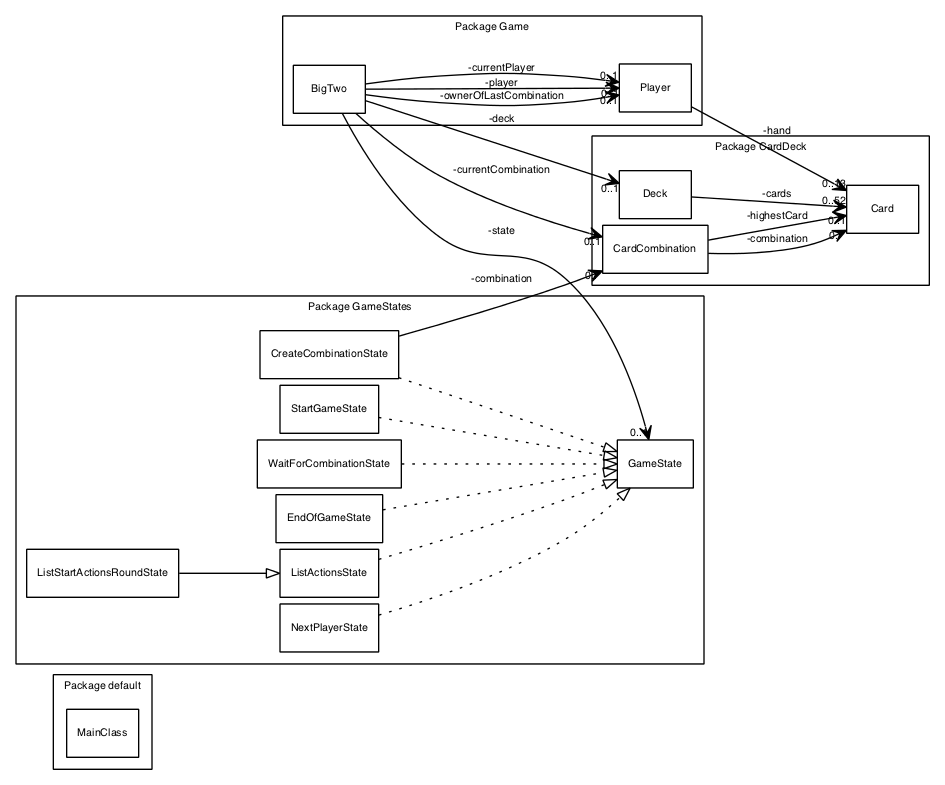
\includegraphics[width=.8\textwidth]{umlsimple.png}
	\caption{Diagrama de classes simplificado}
	\label{uml}
\end{figure}

\vspace{0.8 true cm}

\begin{figure}[h!]
	\centering
	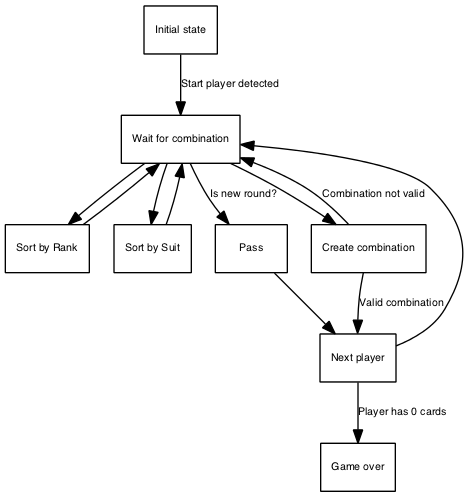
\includegraphics[width=.8\textwidth]{activity.png}
	\caption{Diagrama de atividades}
	\label{activity}
\end{figure}

\section{Classes implementadas}
\label{classesimplementadas}
\vspace{0.4 true cm}
\begin{description}

\item[MainClass] \hfill \\
Classe principal que inicia a execução do jogo.
\vspace{0.4 true cm}

\item[Card] \hfill \\
Classe que contém as informações sobre uma carta, como o seu valor e o naipe, os métodos padrões \textit{getters}, um para o valor e outro para o naipe, além de um método para comprar qual carta é maior.
\vspace{0.4 true cm}

\item[CardCombination] \hfill \\
Classe que lida com todas as combinações possíveis de cada jogada. Possue os métodos que validam se uma determinada combinação é válida e também se uma combinação é maior ou menor que a outra numa comparação.
\vspace{0.4 true cm}

\item[Deck] \hfill \\
Classe que cria uma abstração de um baralho, contendo uma carta de cada valor para cada naipe, o método padrão \textit{get}, além de um método para realizar o embaralhamento das cartas do baralho.
\vspace{0.4 true cm}

\item[BigTwo] \hfill \\
Classe que cuida dos detalhes para inicio do jogo. Contém métodos para a criação dos jogadores, distribuição das cartas entre eles, verifica se a primeira jogada contém o 3 de ouros, cuida da ordem do jogo, quem joga depois de quem, além de \textit{getters} e \textit{setters} padrões.
\vspace{0.4 true cm}

\item[Player] \hfill \\
Classe que representa o jogador. Ele possui uma mão de cartas no jogo, um nome próprio e possui método que pode ordenar suas cartas por naipe ou por valor.
\vspace{0.4 true cm}

\item[CreateCombinationState] \hfill \\
Classe que cuida das mudanças de estado do jogo. Possue métodos que lidam com o fluxo do jogo, sobre a montagem das combinações para as jogadas e se as combinações são válidas para modificar o estado do jogo.
\vspace{0.4 true cm}

\item[EndOfGameState] \hfill \\
Classe que lida com o final do jogo. Realiza a contagem dos pontos e indica o vencedor.
\vspace{0.4 true cm}

\item[ListActionsState] \hfill \\
Classe que lida com os comandos do jogo, quais ações podem ser tomadas para que o jogo continue.
\vspace{0.4 true cm}

\item[ListStartRoundActionsState] \hfill \\
Classe que lida com os comandos da primeira rodada do jogo.
\vspace{0.4 true cm}

\item[NextPlayerState] \hfill \\
Classe que cuida do fluxo de jogadores, ela que determina qual o próximo jogador após cada jogada válida.
\vspace{0.4 true cm}

\item[StartState] \hfill \\
Classe que determina quem é o primeiro jogador da partida.
\vspace{0.4 true cm}

\item[WaitCombinationState] \hfill \\
Classe que cuida da espera por uma ação do jogador.
\vspace{0.4 true cm}

\item[GameState] \hfill \\
Interface que implementa o método de início do jogo.

\end{description}

\subsection{Principais métodos implementados}

Essa subseção irá listar os principais métodos implementados no sistema. Funções triviais não serão listadas, como \textit{getters}, \textit{setters} ou similares. Os métodos detalhados a seguir são os principais utilizados para realizar as comparações entre as cartas, além dos métodos que tratam dos estados possíveis do jogo.

\subsubsection{Card}

\begin{itemize}
\item \begin{large}\textit{public boolean compare(Card that)}\end{large}\\
\subitem \textbf{Descrição:} Realiza a comparação entre duas cartas para determinar qual é maior.
\subitem \textbf{Parâmetros:} Recebe uma carta que se quer comparar com a instância de carta em questão.
\subitem \textbf{Retorno:} Retorna falso se a instância é menor que a carta passada como parametro e verdadeiro se for maior.
\end{itemize}

\vspace{0.2 true cm}

\subsubsection{CardCombination}

\begin{itemize}
\item \begin{large}\textit{public boolean checkCombination()}\end{large}\\
\subitem \textbf{Descrição:} Realiza a chamada do método adequado para verificar se a combinação é válida.
\subitem \textbf{Retorno:} Retorna a chamada de método para cada tipo de combinação e falso para o caso de não ser válida.
\end{itemize}

\vspace{0.2 true cm}

\begin{itemize}
\item \begin{large}\textit{private boolean checkTwoCards()}\end{large}\\
\subitem \textbf{Descrição:} Verifica se a combinação é válida como par.
\subitem \textbf{Retorno:} Retorna verdadeiro se for um par válido e falso se não for um par válido.
\end{itemize}

\vspace{0.2 true cm}

\begin{itemize}
\item \begin{large}\textit{private boolean checkThreeCards()}\end{large}\\
\subitem \textbf{Descrição:} Verifica se a combinação é válida como trinca.
\subitem \textbf{Retorno:} Retorna verdadeiro se for uma trinca válida e falso se não for uma trinca válida.
\end{itemize}

\vspace{0.2 true cm}

\begin{itemize}
\item \begin{large}\textit{private boolean checkFiveCards()}\end{large}\\
\subitem \textbf{Descrição:} Realiza a chamada do método adequado para verificar se a combinação de cinco cartas é válida.
\subitem \textbf{Retorno:} Retorna a chamada de método para cada tipo de combinação de cinco cartas e falso para o caso de não ser válida.
\end{itemize}

\vspace{0.2 true cm}

\begin{itemize}
\item \begin{large}\textit{private boolean checkStraight()}\end{large}\\
\subitem \textbf{Descrição:} Verifica se a combinação é do tipo sequência.
\subitem \textbf{Retorno:} Retorna verdadeiro se for uma sequência válida e falso se não for uma sequência válida.
\end{itemize}

\vspace{0.2 true cm}

\begin{itemize}
\item \begin{large}\textit{private boolean checkFlush()}\end{large}\\
\subitem \textbf{Descrição:} Verifica se a combinação é do tipo flush.
\subitem \textbf{Retorno:} Retorna verdadeiro se for um flush válido e falso se não for um flush válido.
\end{itemize}

\vspace{0.2 true cm}

\begin{itemize}
\item \begin{large}\textit{private boolean checkFullHouse()}\end{large}\\
\subitem \textbf{Descrição:} Verifica se a combinação é do tipo full house.
\subitem \textbf{Retorno:} Retorna verdadeiro se for um full house válido e falso se não for um full house válido.
\end{itemize}

\vspace{0.2 true cm}

\begin{itemize}
\item \begin{large}\textit{private boolean checkFour()}\end{large}\\
\subitem \textbf{Descrição:} Verifica se a combinação é do tipo four.
\subitem \textbf{Retorno:} Retorna verdadeiro se for um four válido e falso se não for um four válido.
\end{itemize}

\vspace{0.2 true cm}

\begin{itemize}
\item \begin{large}\textit{private boolean checkThreeOfDiamonds()}\end{large}\\
\subitem \textbf{Descrição:} Verifica se na combinação existe o 3 de ouros.
\subitem \textbf{Retorno:} Retorna verdadeiro se existir o 3 de ouros na combinação e falso se não existir.
\end{itemize}

\vspace{0.2 true cm}

\begin{itemize}
\item \begin{large}\textit{public boolean checkFirstCombination()}\end{large}\\
\subitem \textbf{Descrição:} Verifica se a primeira combinação do jogo é válida e se ela possui o 3 de ouros.
\subitem \textbf{Retorno:} Retorna verdadeiro se for válido e existir o 3 de ouros na combinação e falso se algum dos dois for falso.
\end{itemize}

\vspace{0.2 true cm}

\begin{itemize}
\item \begin{large}\textit{private void sortByRank()}\end{large}\\
\subitem \textbf{Descrição:} Realiza a ordenação das cartas da combinação por valor.
\end{itemize}

\vspace{0.2 true cm}

\begin{itemize}
\item \begin{large}\textit{public void sortBySuit()}\end{large}\\
\subitem \textbf{Descrição:} Realiza a ordenação das cartas da combinação por naipe.
\end{itemize}

\vspace{0.2 true cm}

\begin{itemize}
\item \begin{large}\textit{public boolean isHigherThan(CardCombination that)}\end{large}\\
\subitem \textbf{Descrição:} Realiza a comparação entre duas combinações de cartas para determinar qual é maior.
\subitem \textbf{Parâmetros:} Recebe uma combinação que se quer comparar com a instância de combinação em questão.
\subitem \textbf{Retorno:} Retorna falso se a instância é menor que a combinação passada como parâmetro e verdadeiro se for maior.
\end{itemize}

\vspace{0.2 true cm}

\subsubsection{Deck}

\begin{itemize}
\item \begin{large}\textit{public void shuffle()}\end{large}\\
\subitem \textbf{Descrição:} Realiza o embaralhamento das cartas utilizando uma função padrão do Java para lidar com Collections.
\end{itemize}

\vspace{0.2 true cm}

\subsubsection{BigTwo}

\begin{itemize}
\item \begin{large}\textit{public void startGame()}\end{large}\\
\subitem \textbf{Descrição:} Chama os métodos que de fato inicia o jogo.
\end{itemize}

\vspace{0.2 true cm}

\begin{itemize}
\item \begin{large}\textit{private void createPlayers()}\end{large}\\
\subitem \textbf{Descrição:} Realiza a criação dos 4 jogadores.
\end{itemize}

\vspace{0.2 true cm}

\begin{itemize}
\item \begin{large}\textit{private void distributeCards()}\end{large}\\
\subitem \textbf{Descrição:} Realiza a distribuição das cartas para os jogadores, cada um com 13 cartas.
\end{itemize}

\vspace{0.2 true cm}

\begin{itemize}
\item \begin{large}\textit{public void setNextPlayer()}\end{large}\\
\subitem \textbf{Descrição:} Determina qual o jogador da próxima rodada.
\end{itemize}

\vspace{0.2 true cm}

\begin{itemize}
\item \begin{large}\textit{public void printCurrentCombination()}\end{large}\\
\subitem \textbf{Descrição:} Imprime na tela a combinação que está na mesa atualmente e que deve ser vencida para que se possa jogar.
\end{itemize}

\vspace{0.2 true cm}

\begin{itemize}
\item \begin{large}\textit{public boolean gameOver()}\end{large}\\
\subitem \textbf{Descrição:} Verifica se algum jogador terminou suas cartas, imprime que o jogo acabou.
\subitem \textbf{Retorno:} Retorna verdadeiro se o algum jogador terminou suas carta e falso caso contrário.
\end{itemize}

\vspace{0.2 true cm}

\begin{itemize}
\item \begin{large}\textit{public void updateLowestHand(Player p)}\end{large}\\
\subitem \textbf{Descrição:} Atualiza para cada jogador para sempre ficar armazenado qual jogador tem o menor número de cartas do jogo.
\subitem \textbf{Parâmetro:} Recebe como parâmetro o jogador que acabou de jogar.
\end{itemize}

\vspace{0.2 true cm}

\subsubsection{CreateCombinationState}

\begin{itemize}
\item \begin{large}\textit{public void doAction(BigTwo game)}\end{large}\\
\subitem \textbf{Descrição:} Realiza o controle da criação de uma combinação para ser jogada.
\subitem \textbf{Parâmetro:} Recebe como parâmetro o próprio jogo.
\end{itemize}

\vspace{0.2 true cm}

\begin{itemize}
\item \begin{large}\textit{public void listHand(BigTwo game)}\end{large}\\
\subitem \textbf{Descrição:} Realiza a impressão das opções de cartas e um índice de escolhas.
\subitem \textbf{Parâmetro:} Recebe como parâmetro o próprio jogo.
\end{itemize}

\vspace{0.2 true cm}

\begin{itemize}
\item \begin{large}\textit{public void playCombination(BigTwo game)}\end{large}\\
\subitem \textbf{Descrição:} Realiza o controle da jogada em si, chamando os métodos para validar a jogada.
\subitem \textbf{Parâmetro:} Recebe como parâmetro o próprio jogo.
\end{itemize}

\vspace{0.2 true cm}

\begin{itemize}
\item \begin{large}\textit{public boolean createCombination()}\end{large}\\
\subitem \textbf{Descrição:} Realiza o controle da formação da combinação, ao selecionar carta por carta.
\subitem \textbf{Parâmetro:} Recebe como parâmetro o próprio jogo.
\subitem \textbf{Retorno:} Retorna verdadeiro se a combinação foi criada com sucesso e falso caso contrário.
\end{itemize}

\vspace{0.2 true cm}

\begin{itemize}
\item \begin{large}\textit{public boolean setSizeOfCombination()}\end{large}\\
\subitem \textbf{Descrição:} Determina o tamanho da combinação a ser formada em seguida.
\subitem \textbf{Retorno:} Retorna verdadeiro se o tamanho da combinação for válida e falso caso contrário.
\end{itemize}

\vspace{0.2 true cm}

\begin{itemize}
\item \begin{large}\textit{public boolean confirmCombination()}\end{large}\\
\subitem \textbf{Descrição:} Realiza o controle da validação da jogada, verificando todos os detalhes para a jogada ser válida.
\subitem \textbf{Retorno:} Retorna verdadeiro se a combinação for jogada com sucesso e falso caso contrário.
\end{itemize}

\vspace{0.2 true cm}

\begin{itemize}
\item \begin{large}\textit{public void checkCombination(BigTwo game)}\end{large}\\
\subitem \textbf{Descrição:} Verifica se a combinação é válida, sobretudo se for a primeira rodada do jogo.
\subitem \textbf{Parâmetro:} Recebe como parâmetro o próprio jogo.
\end{itemize}

\vspace{0.2 true cm}

\begin{itemize}
\item \begin{large}\textit{public void removeCombinationFromHand(BigTwo game)}\end{large}\\
\subitem \textbf{Descrição:} Remove as cartas da combinação jogada da mão do jogador.
\subitem \textbf{Parâmetro:} Recebe como parâmetro o próprio jogo.
\end{itemize}

\vspace{0.2 true cm}

\subsubsection{EndOfGameState}

\begin{itemize}
\item \begin{large}\textit{public void doAction(BigTwo game)}\end{large}\\
\subitem \textbf{Descrição:} Imprime que o jogo acabou e quem foi o vencedor.
\subitem \textbf{Parâmetro:} Recebe como parâmetro o próprio jogo.
\end{itemize}

\vspace{0.2 true cm}

\subsubsection{ListActionsState}

\begin{itemize}
\item \begin{large}\textit{public void doAction(BigTwo game)}\end{large}\\
\subitem \textbf{Descrição:} Realiza o controle da ação de escolha do comando.
\subitem \textbf{Parâmetro:} Recebe como parâmetro o próprio jogo.
\end{itemize}

\vspace{0.2 true cm}

\begin{itemize}
\item \begin{large}\textit{public int waitingForInput()}\end{large}\\
\subitem \textbf{Descrição:} Espera pelo comando do usuário.
\subitem \textbf{Retorno:} Retorna o inteiro que representa o comando escolhido.
\end{itemize}

\vspace{0.2 true cm}

\begin{itemize}
\item \begin{large}\textit{public void listActions()}\end{large}\\
\subitem \textbf{Descrição:} Lista os comandos possíveis.
\end{itemize}

\vspace{0.2 true cm}

\begin{itemize}
\item \begin{large}\textit{public GameState nextState(int action, BigTwo game)}\end{large}\\
\subitem \textbf{Descrição:} Realiza o controle do estado, modificando ele de acordo com o comando.
\subitem \textbf{Parâmetro:} Recebe como parâmetro o próprio jogo e o inteiro com o comando.
\subitem \textbf{Retorno:} Retorna o estado do jogo.
\end{itemize}

\vspace{0.2 true cm}

\subsubsection{ListStartRoundActionsState}

\begin{itemize}
\item \begin{large}\textit{public void listActions()}\end{large}\\
\subitem \textbf{Descrição:} Lista os comandos possíveis.
\end{itemize}

\vspace{0.2 true cm}

\begin{itemize}
\item \begin{large}\textit{public GameState nextState(int action, BigTwo game)}\end{large}\\
\subitem \textbf{Descrição:} Realiza o controle do estado, modificando ele de acordo com o comando.
\subitem \textbf{Parâmetro:} Recebe como parâmetro o próprio jogo e o inteiro com o comando.
\subitem \textbf{Retorno:} Retorna o estado do jogo.
\end{itemize}

\vspace{0.2 true cm}

\subsubsection{NextPlayerState}

\begin{itemize}
\item \begin{large}\textit{public void doAction(BigTwo game)}\end{large}\\
\subitem \textbf{Descrição:} Realiza a mudança do jogador atual depois de uma jogada.
\subitem \textbf{Parâmetro:} Recebe como parâmetro o próprio jogo.
\end{itemize}

\vspace{0.2 true cm}

\subsubsection{StartState}

\begin{itemize}
\item \begin{large}\textit{public void doAction(BigTwo game)}\end{large}\\
\subitem \textbf{Descrição:} Realiza o controle do inicio do jogo, imprimindo o primeiro jogador.
\subitem \textbf{Parâmetro:} Recebe como parâmetro o próprio jogo.
\end{itemize}

\vspace{0.2 true cm}

\subsubsection{WaitCombinationState}

\begin{itemize}
\item \begin{large}\textit{public void doAction(BigTwo game)}\end{large}\\
\subitem \textbf{Descrição:} Realiza a espera pela próxima ação do próximo jogador.
\subitem \textbf{Parâmetro:} Recebe como parâmetro o próprio jogo.
\end{itemize}

\vspace{0.2 true cm}

\section{Testes}
\label{testes}
Para esse trabalho, os testes foram os mais legais possíveis, pois testamos o jogo jogando! Não criamos nenhum teste automatizado, mas criamos uma planilha de BUGs para serem resolvidos. Para fins de demonstração, imprimimos uma rodada do jogo para ilustrar como ficou a interação do jogador.

\subsection{Listagem da saída}

\begin{verbatim}

Starting game...
Shuffling the deck...
Creating players...
Distributing cards...
Player 2's plays first.
Waiting for Player 2's action...
Player 2 choose your action:
1) Sort hand by suit
2) Sort hand by rank
3) Create combination of cards
Selection your action...
2
Sorting hand by rank...
Current hand...
THREE of SPADES
THREE of DIAMONDS
FOUR of HEARTS
SEVEN of CLUBS
SEVEN of SPADES
EIGHT of SPADES
EIGHT of CLUBS
TEN of CLUBS
JACK of DIAMONDS
ACE of CLUBS
ACE of HEARTS
ACE of DIAMONDS
TWO of SPADES
Player 2 choose your action:
1) Sort hand by suit
2) Sort hand by rank
3) Create combination of cards
Selection your action...
3
Choices of cards...
[ 1 ] THREE of SPADES
[ 2 ] THREE of DIAMONDS
[ 3 ] FOUR of HEARTS
[ 4 ] SEVEN of CLUBS
[ 5 ] SEVEN of SPADES
[ 6 ] EIGHT of SPADES
[ 7 ] EIGHT of CLUBS
[ 8 ] TEN of CLUBS
[ 9 ] JACK of DIAMONDS
[ 10 ] ACE of CLUBS
[ 11 ] ACE of HEARTS
[ 12 ] ACE of DIAMONDS
[ 13 ] TWO of SPADES
How many cards will you combination have? (1, 2, 3 or 5)
(press any letter to go back to actions)
2
Enter next card: 
1
Enter next card: 
2
Pair
THREE of DIAMONDS
THREE of SPADES
Play this combination? (y/n)
y
Current hand...
FOUR of HEARTS
SEVEN of CLUBS
SEVEN of SPADES
EIGHT of SPADES
EIGHT of CLUBS
TEN of CLUBS
JACK of DIAMONDS
ACE of CLUBS
ACE of HEARTS
ACE of DIAMONDS
TWO of SPADES
--------------------------------
Waiting for Player 3's action...
Player 3 choose your action:
1) Sort hand by suit
2) Sort hand by rank
3) Create combination of cards
4) Pass
Selection your action...

\end{verbatim}

\section{Conclusão}
\label{conclusao}

O trabalho prático foi prazeroso de ser realizado. Os conceitos de modelagem de classe aprendidos em sala foram bastante reforçados quando nos deparamos com um problema complexo como este.

Foi necessário lidar com o desafio de não ter uma especificação detalhada, o que traz uma série de dificuldades e decições complicadas de serem tomadas. Apesar disso, foi muito interessante e acreditamos que a escolha de um jogo como tema livre proporcionou uma motivação a mais para os alunos do que se fosse um assunto menos divertido. 

\bibliographystyle{sbc}
\bibliography{tp1}

\begin{figure}[h!]
	\centering
	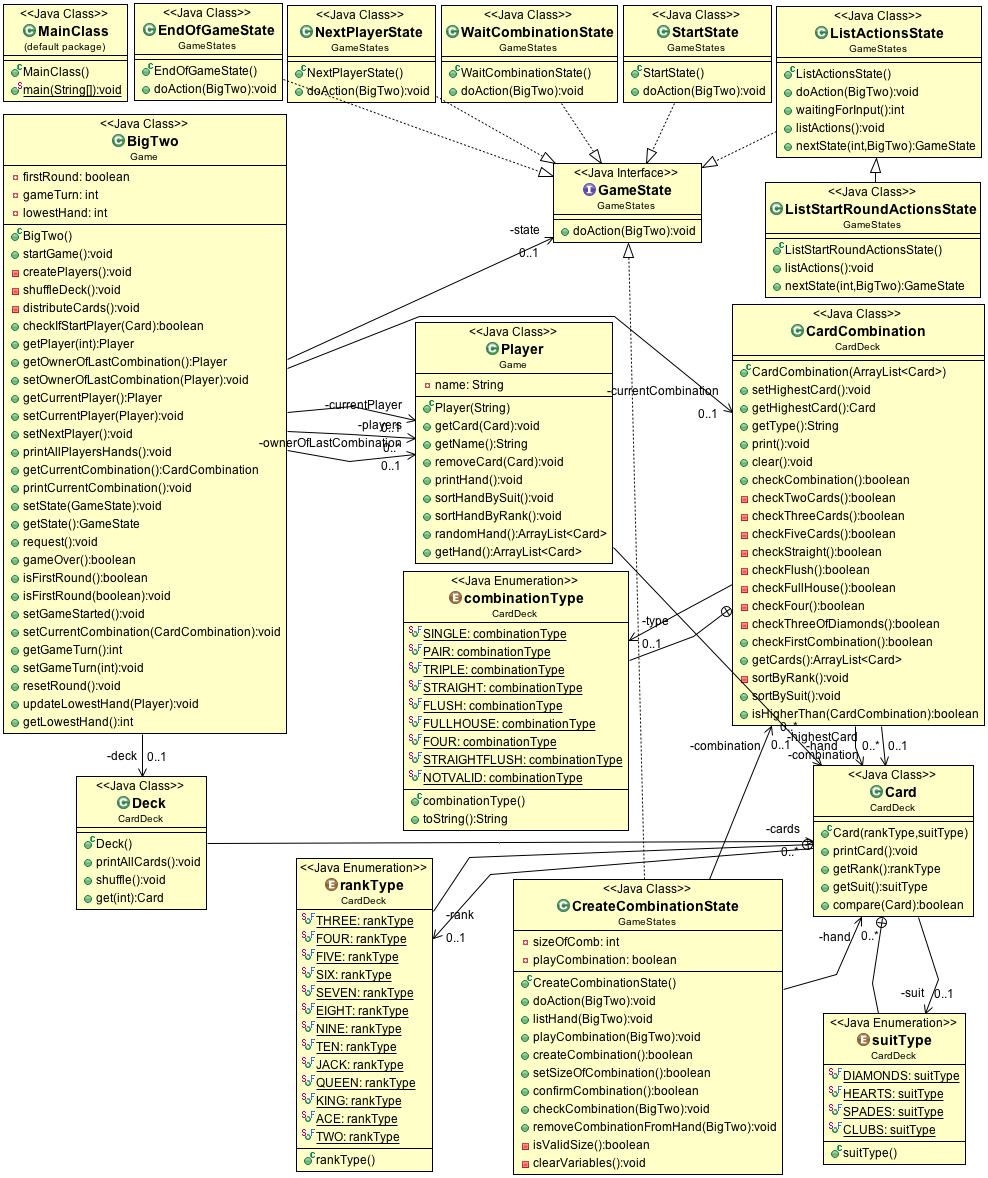
\includegraphics[width=.8\textwidth]{umlfull.png}
	\caption{Diagrama de classes completo}
	\label{umlfull}
\end{figure}

\end{document}
